\documentclass{article}
\usepackage[utf8]{inputenc}
\usepackage{amsmath}
\usepackage{mathtools}
\usepackage{float}
\usepackage[numbered, framed]{matlab-prettifier}
\usepackage[font=small]{caption}

\setlength{\abovecaptionskip}{3pt}
\setlength{\belowcaptionskip}{3pt}

\title{Control Theory Homework 3}
\author{Kamil Kamaliev, Var e \\ k.kamaliev@innopolis.university}
\date{March 2020}

\begin{document}

\maketitle

\paragraph{Exercise 3.}

$$ W = \frac{s + 2}{2s^2 + 7} $$

\begin{figure}[hbt!]
        \centering
        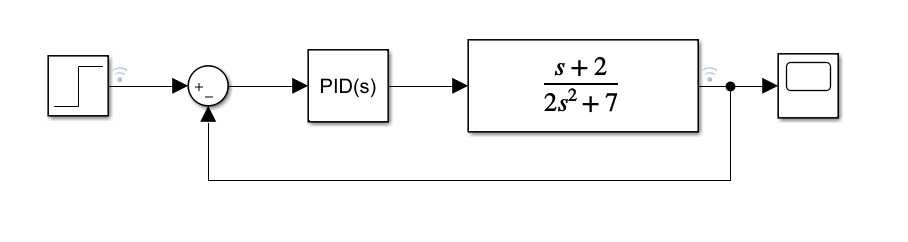
\includegraphics[scale=0.4]{hw3_3schema.png}
        \caption{Simulink Schema}
\end{figure}

I decided to start with $k_p = 1 \ and \ k_d = k_i = 0$

\begin{figure}[hbt!]
        \centering
        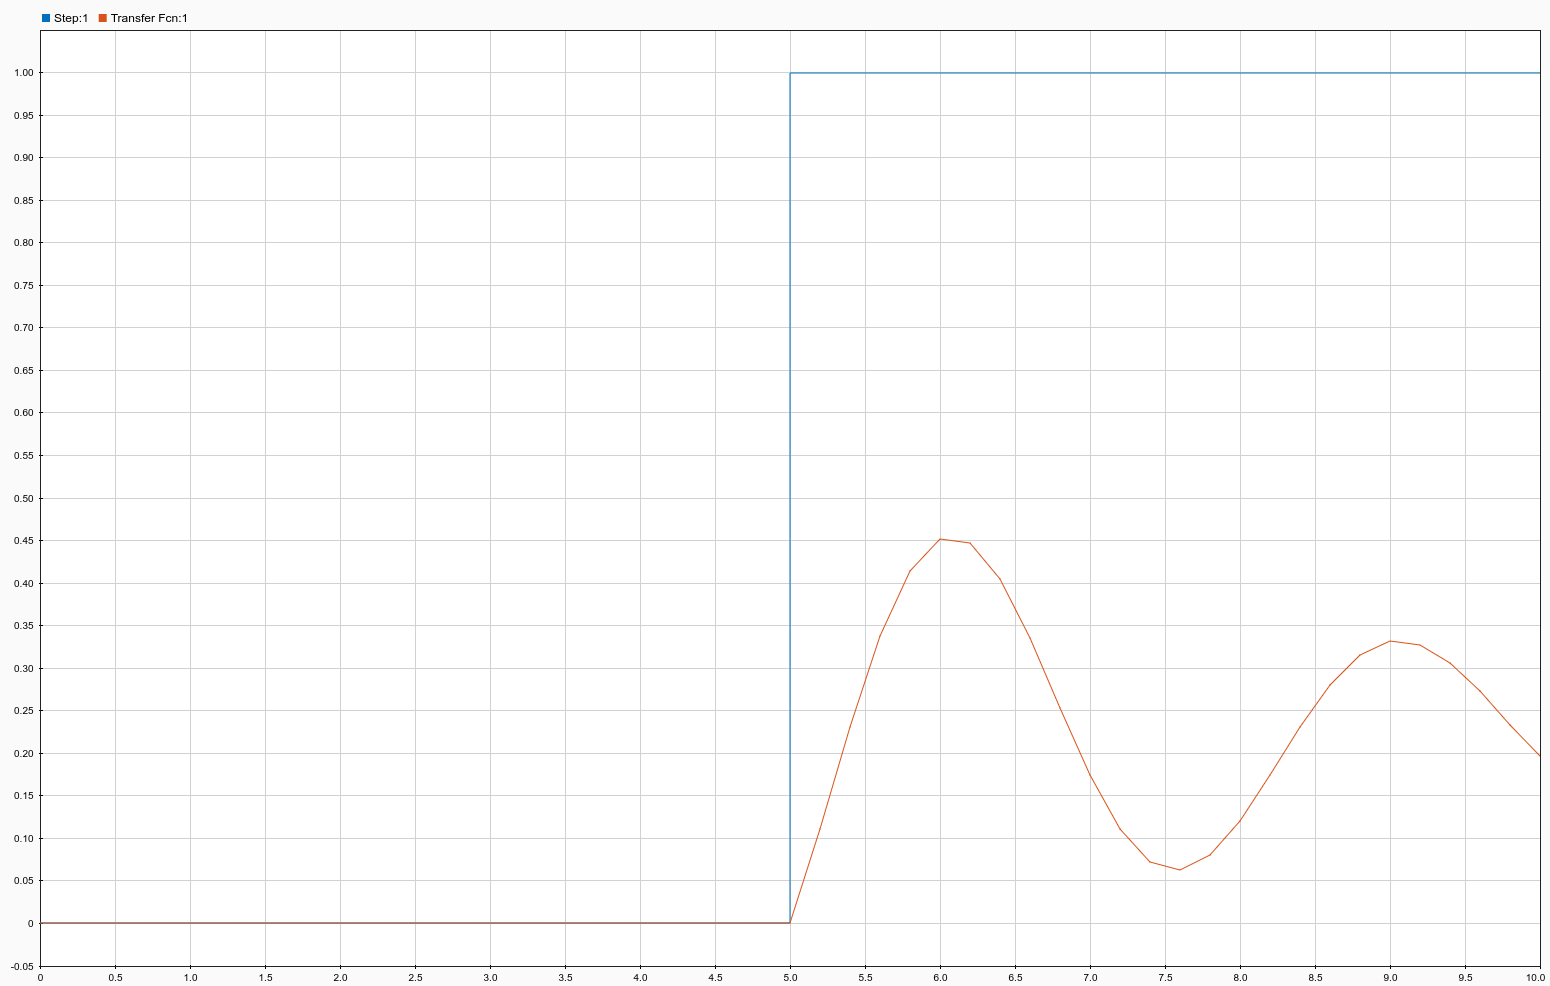
\includegraphics[scale=0.2]{hw3_3no_cont.png}
        \caption{$k_p = 1 \ and \ k_d = k_i = 0$}
\end{figure}

As we can see, the system is far from the desired control.

To solve this problem, I adjusted the the coefficients using PID Tuner.

\newpage

\begin{figure}[hbt!]
        \centering
        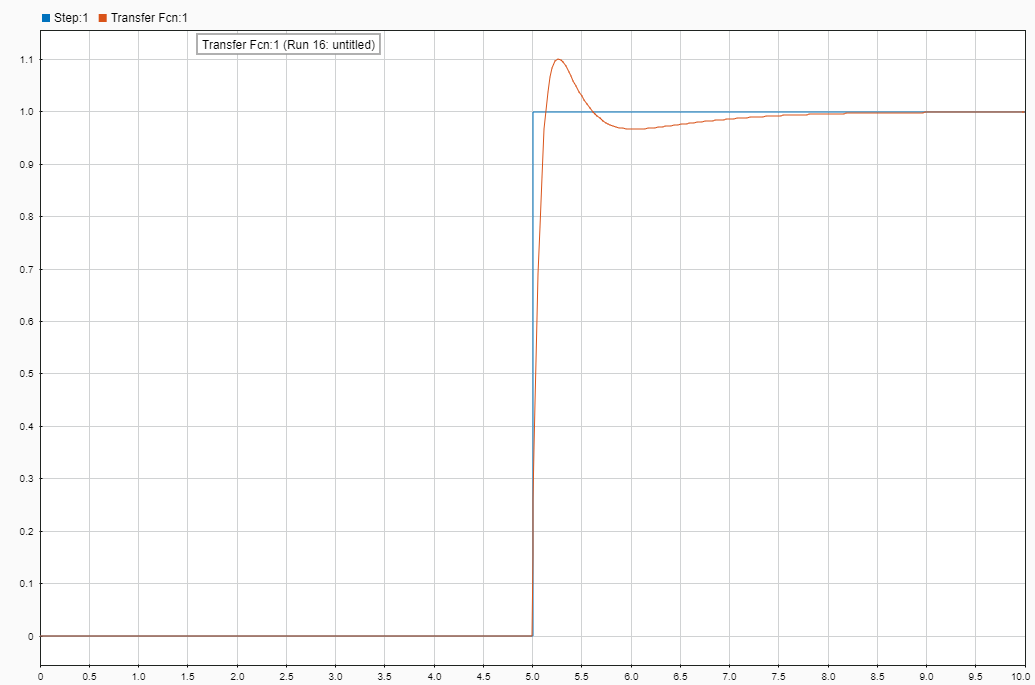
\includegraphics[scale=0.3]{hw3_3overshoot.png}
        \caption{Overshoot with $k_p = 35, \ k_d = 0.4, \ k_i = 61$}
\end{figure}

\noindent
The controller above stabilize the system pretty fast. However, it overshoots.


\begin{figure}[hbt!]
        \centering
        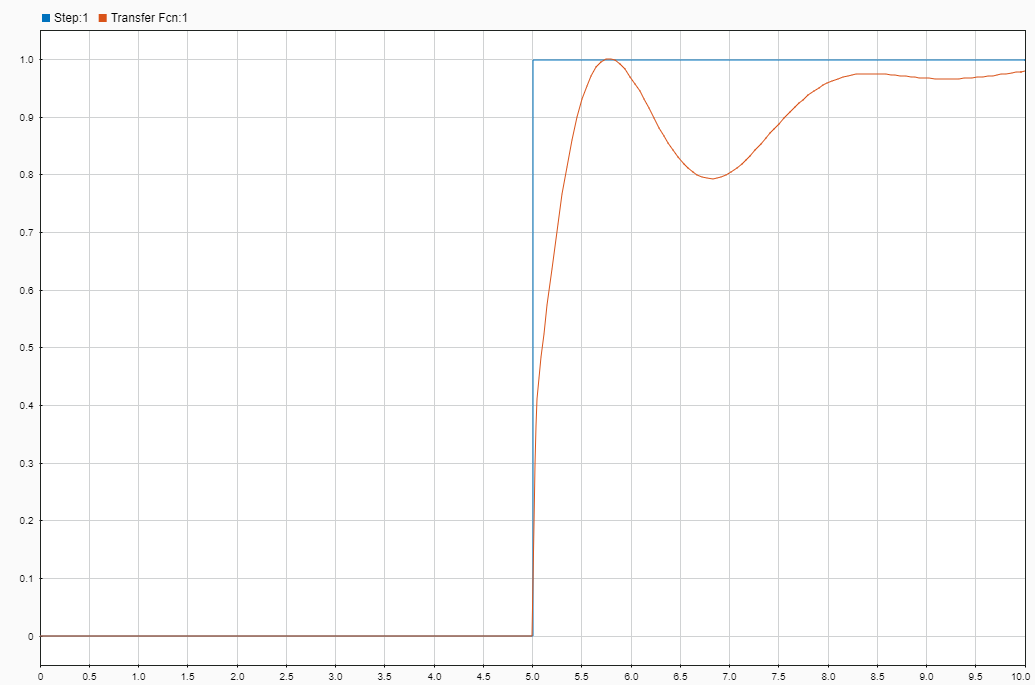
\includegraphics[scale=0.3]{hw3_3no_overshoot.png}
        \caption{No overshoot with $k_p = 5.33, \ k_d = 0.99, \ k_i = 6.75$}
\end{figure}

\noindent
The controller above doesn't overshoot. However, its stabilization time is greater than the one that the previous controller had.

\smallbreak

\noindent
As a result, we need to make choice between overshooting and minimizing the stabilization time.

\newpage

\paragraph{Exercise 4.}

$$ W(s) = \frac{s + 4}{s^2 + 3s + 15}$$

\noindent
Afer openning the Matlab Control System Designer, we see the following picture:

\begin{figure}[hbt!]
        \centering
        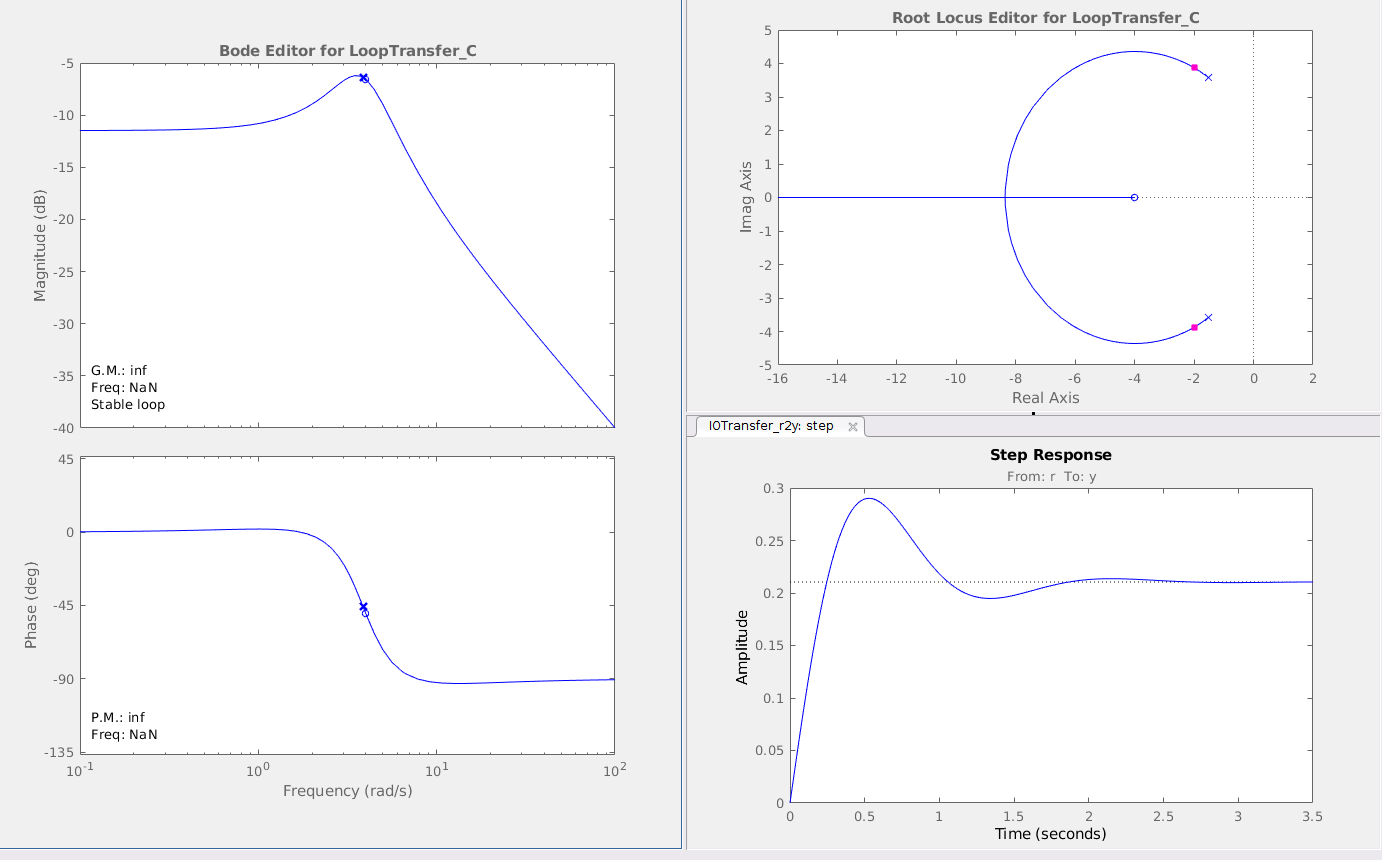
\includegraphics[scale=0.3]{hw3_41.png}
        \caption{Original System}
\end{figure}

To make orientation easier the following design requirements were set: 

\noindent
rise\_time=1, settle\_time=3, overshoot=20\%

\bigbreak
Then,  in order to make it rise to 1, I added integrator (real pole in zero) and, to decrease the rise time, adjusted the bode magnitude plot

\newpage

\noindent
After the described manipulations I obtained the following:

\begin{figure}[hbt!]
        \centering
        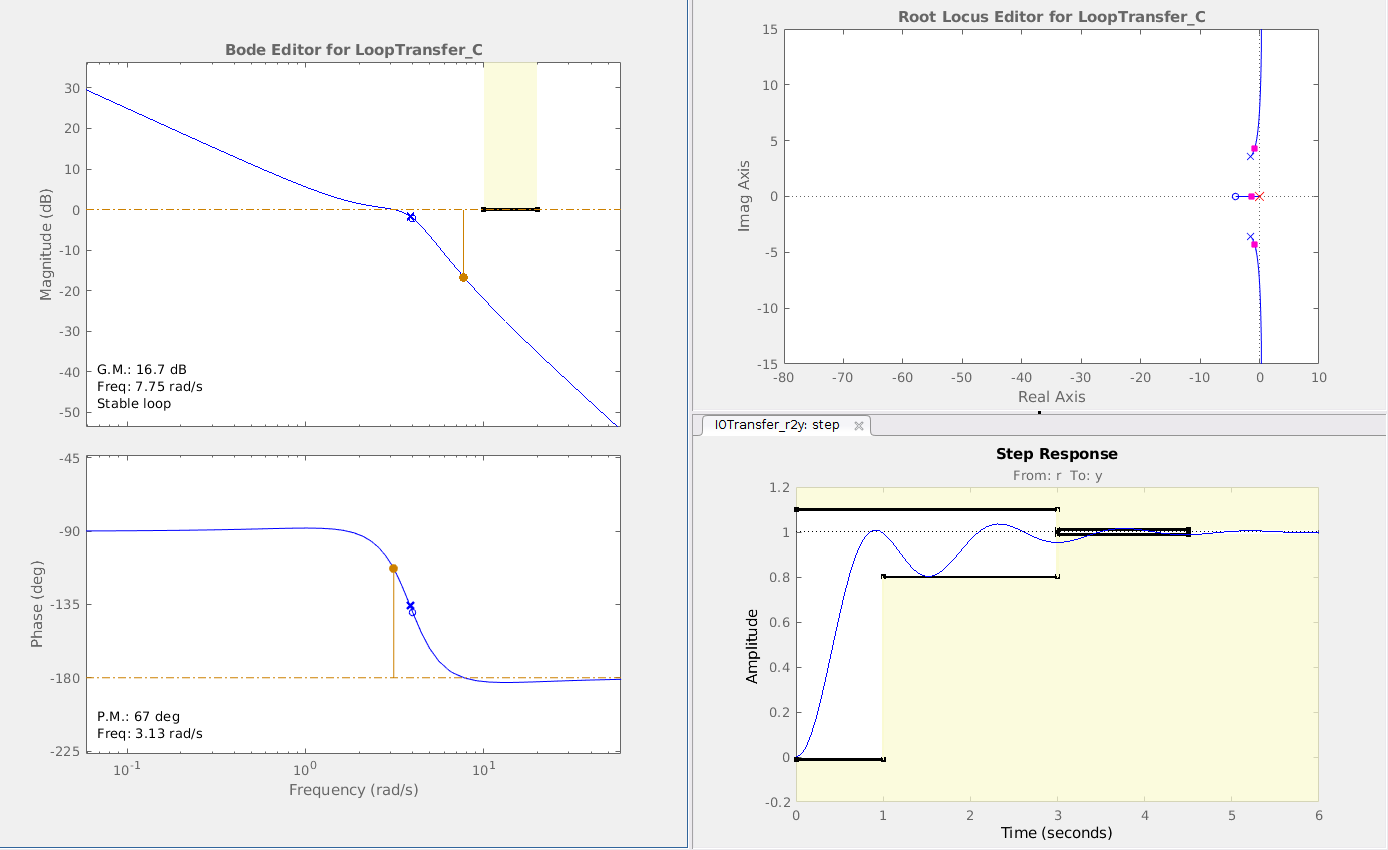
\includegraphics[scale=0.3]{hw3_42.png}
        \caption{System with integrator and adjusted bode plot}
\end{figure}


\noindent
To get rid of overshoot and decrease the stabilization time, I added several real zeroes and symmetric complex pole

\begin{figure}[hbt!]
        \centering
        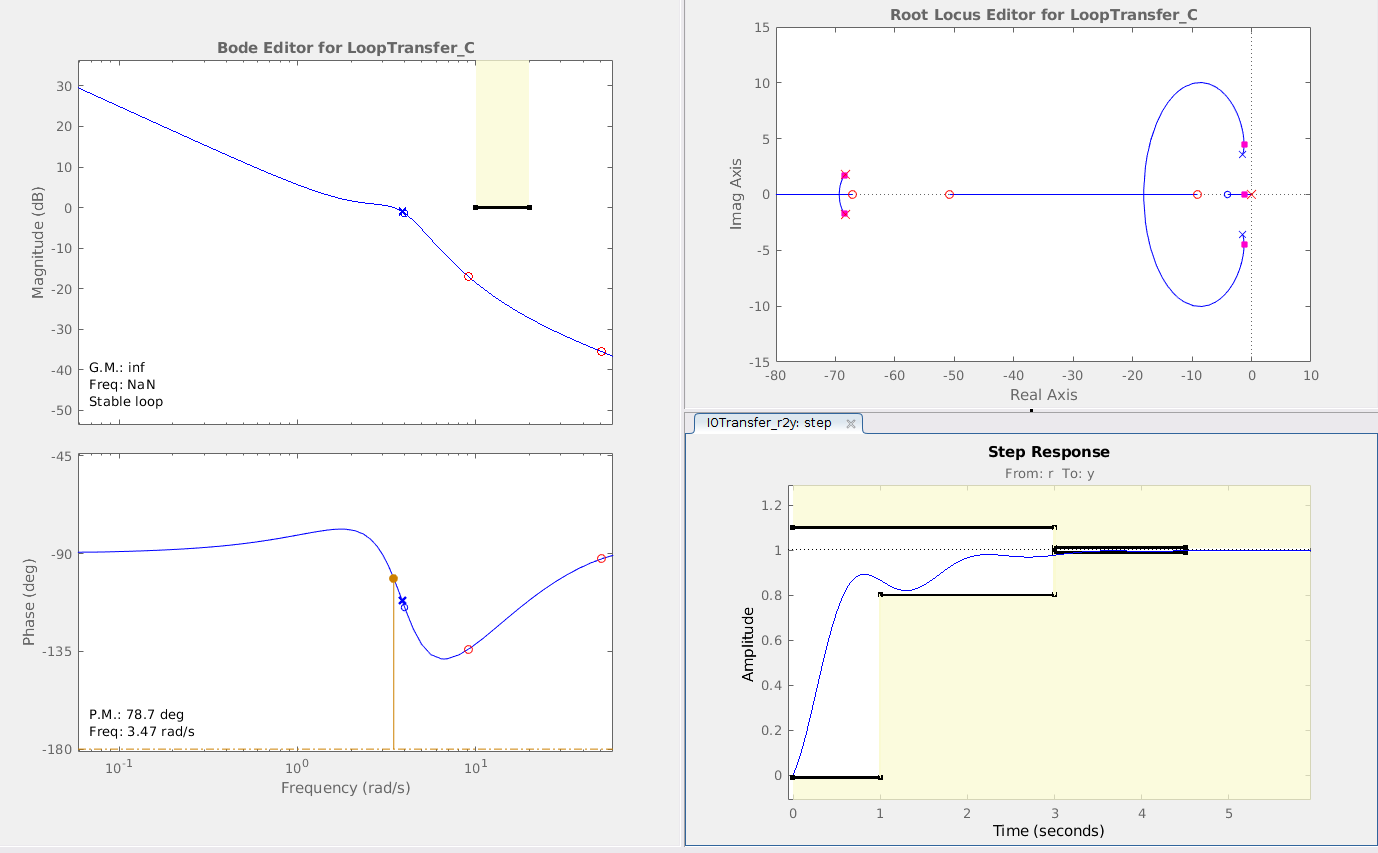
\includegraphics[scale=0.3]{hw3_43.png}
        \caption{System with integrator and adjusted bode plot}
\end{figure}


\end{document}